\documentclass[crop, tikz]{standalone}
\RequirePackage{luatex85}

\usepackage{fontawesome}
\usepackage{fontspec}
\usetikzlibrary{
    shapes,
    arrows,
    arrows.meta,
    positioning,
    decorations.pathmorphing,
    shapes.geometric,
    decorations.pathreplacing
}

\newfontfamily{\ttfamily}{Fira Code}
\usepackage{fontspec}
\setmainfont{Liberation Sans}
\newfontfamily\ExtraLight{Liberation Sans}
\newfontfamily\Light{Liberation Sans}
\newfontfamily\Book{Liberation Sans}
\newfontfamily\Medium{Liberation Sans}

\makeatletter
\tikzset{arrow-pointer-up/.style={
        single arrow,
        minimum height=1.5cm,
        inner sep=5pt,
        line width=1pt,
        draw,
        color=gray,
        single arrow head extend=0.1cm,
        rotate=90,
        %single arrow tip angle=90,
        %shape border rotate=90,
        %shape border uses incircle,
    }
}

\tikzset{arrow-pointer-down/.style={
        single arrow,
        minimum height=1.5cm,
        inner sep=5pt,
        line width=1pt,
        draw,
        color=gray,
        rotate=-90,
        %single arrow tip angle=90,
        %shape border rotate=-90,
        %shape border uses incircle,
        single arrow head extend=0.1cm
    }
}

\tikzset{
    database/.style={
        path picture={
            \draw (0, 1.5*\database@segmentheight) circle [x radius=\database@radius,y radius=\database@aspectratio*\database@radius];
            \draw (-\database@radius, 0.5*\database@segmentheight) arc [start angle=180,end angle=360,x radius=\database@radius, y radius=\database@aspectratio*\database@radius];
            \draw (-\database@radius,-0.5*\database@segmentheight) arc [start angle=180,end angle=360,x radius=\database@radius, y radius=\database@aspectratio*\database@radius];
            \draw (-\database@radius,1.5*\database@segmentheight) -- ++(0,-3*\database@segmentheight) arc [start angle=180,end angle=360,x radius=\database@radius, y radius=\database@aspectratio*\database@radius] -- ++(0,3*\database@segmentheight);
        },
        minimum width=4*\database@radius + \pgflinewidth,
        minimum height=3*\database@segmentheight + 2*\database@aspectratio*\database@radius + \pgflinewidth,
    },
    database segment height/.store in=\database@segmentheight,
    database radius/.store in=\database@radius,
    database aspect ratio/.store in=\database@aspectratio,
    database segment height=1.5cm,
    database radius=2.5cm,
    database aspect ratio=0.35,
}
\makeatother

\begin{document}
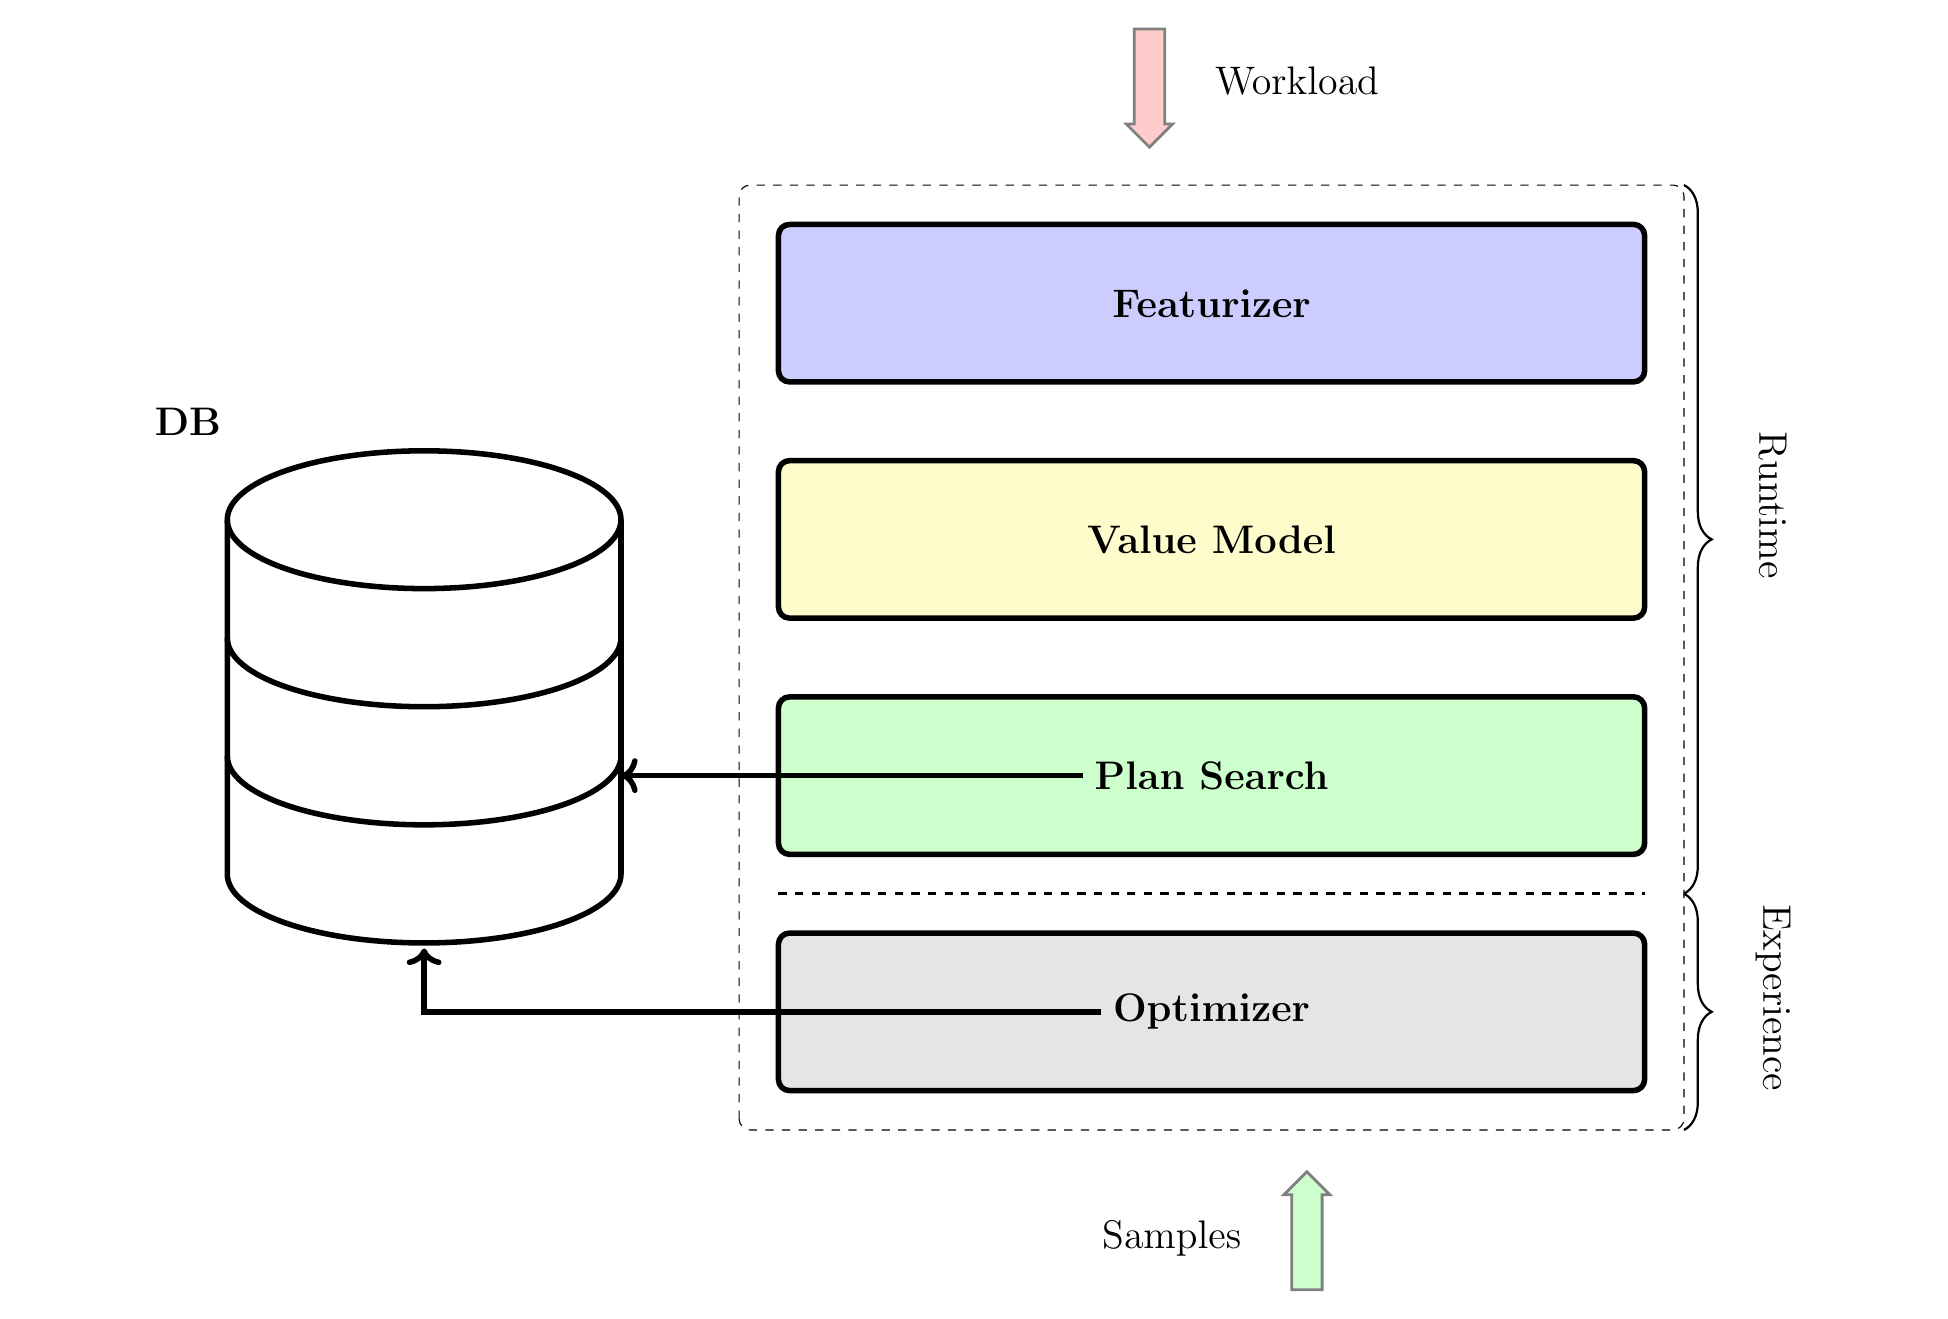
\begin{tikzpicture}[
    queue/.style={},
    connection/.style={-,>=stealth',semithick,rounded corners=5pt}
    ]

    \path[] (0.0, 0.0) rectangle (15, 12.5) {};
    \node[solid,database,label={[xshift=-3cm]\Large{\textbf{DB}}}, line width=2pt] at (-4.0, 6.0) (database) {};
    \coordinate (to-db) at (-1.5, 5.0);

    \draw[rounded corners, dashed] (0, 0.5) rectangle (12, 12.5) node[pos=0.5] {};
    \draw[rounded corners, line width=2pt, fill=blue!20] (0.5, 10.0) rectangle (11.5, 12.0) node[pos=0.5] (featurizer) {\Large{\textbf{Featurizer}}};
    \draw[rounded corners, line width=2pt, fill=yellow!20] (0.5, 7.0) rectangle (11.5, 9.0) node[pos=0.5] (model) {\Large{\textbf{Value Model}}};
    \draw[rounded corners, line width=2pt, fill=green!20] (0.5, 4.0) rectangle (11.5, 6.0) node[pos=0.5] (plan-search) {\Large{\textbf{Plan Search}}};
    \draw[rounded corners, line width=2pt, fill=gray!20] (0.5, 1.0) rectangle (11.5, 3.0) node[pos=0.5] (optimizer) {\Large{\textbf{Optimizer}}};
    \draw[draw, dashed, line width=1.0] (0.5, 3.5) -- (11.5, 3.5);
    \node[arrow-pointer-up, below=2.5cm of optimizer.south, label={[label distance=0.5cm]\Large{Samples}}, yshift=-1cm, fill=green!20] {};
    \node[arrow-pointer-down, above=2.5cm of featurizer.north, label={[label distance=0.5cm]\Large{Workload}}, yshift=-1cm, fill=red!20] {};

    \draw[thick, decorate, decoration={brace, amplitude=10pt, mirror}] (12, 0.5) -- +(0, 3.0)
           node[black, midway, font=\Large, rotate=-90, label={[label distance=0.5cm, rotate=-90, xshift=-2cm, yshift=1cm]\Large{Experience}}] {};

    \draw[thick, decorate, decoration={brace, amplitude=10pt, mirror}] (12, 3.5) -- +(0, 9.0)
           node[black, midway, font=\Large, rotate=-90, label={[label distance=0.5cm, rotate=-90, xshift=-2cm, yshift=1cm]\Large{Runtime}}] {};

    \draw[->, line width=2pt] (optimizer) -| (database.south);
    \draw[->, line width=2pt] (plan-search) -- (to-db);

\end{tikzpicture}
\end{document}
